\documentclass[table]{beamer}

\title{Using the internal language of toposes in algebraic geometry}
\author{Ingo Blechschmidt}
\institute{University of Augsburg}
\date{June 23th, 2014}

\usepackage[english]{babel}
\usepackage[protrusion=true,expansion=true]{microtype}
\usepackage{amsmath,amsfonts,amssymb,amsthm}
\usepackage{tikz}
\usepackage{booktabs}
\usepackage{ragged2e}
\usepackage[orientation=landscape,size=a2,scale=0.8]{beamerposter}

\usefonttheme{professionalfonts}
\usepackage{pxfonts}

\definecolor{lgreen} {RGB}{180,210,100}
\definecolor{dblue}  {RGB}{20,66,129}
\definecolor{ddblue} {RGB}{11,36,69}
\definecolor{lred}   {RGB}{220,0,0}
\definecolor{nred}   {RGB}{224,0,0}
\definecolor{norange}{RGB}{230,120,20}
\definecolor{nyellow}{RGB}{255,221,0}
\definecolor{ngreen} {RGB}{98,158,31}
\definecolor{dgreen} {RGB}{78,138,21}
\definecolor{nblue}  {RGB}{28,130,185}
\definecolor{jblue}  {RGB}{20,50,100}

\setbeamercolor{palette primary}   {fg=black,bg=white}
\setbeamercolor{palette secondary} {fg=black,bg=white}
\setbeamercolor{palette tertiary}  {bg=jblue,fg=white}
\setbeamercolor{palette quaternary}{fg=black,bg=white}
\setbeamercolor{structure}{fg=jblue}
\setbeamercolor{titlelike}         {bg=jblue,fg=white}
\setbeamercolor{frametitle}        {bg=jblue!10,fg=jblue}
\setbeamercolor{cboxb}{fg=black,bg=jblue}
\setbeamercolor{cboxr}{fg=black,bg=red}

\setbeamercolor{item}{fg=ngreen}
\setbeamercolor{item projected}{fg=white,bg=ngreen}

\setbeamercolor{block title}{fg=nred,bg=white}
\setbeamercolor{block body}{fg=black,bg=white}

\setbeamercolor{block alerted title}{fg=white,bg=jblue}
\setbeamercolor{block alerted body}{fg=black,bg=jblue!10}

\setbeamerfont{section in head/foot}{series=\bfseries}
\setbeamerfont{block title}{series=\bfseries}
\setbeamerfont{block alerted title}{series=\bfseries}
\setbeamerfont{frametitle}{series=\bfseries}
\setbeamerfont{frametitle}{size=\Large}
\setbeamerfont{block body}{series=\rmfamily}

\setbeamertemplate{items}[circle]
\setbeamertemplate{blocks}[width=0.0]
\beamertemplatenavigationsymbolsempty

\setbeamertemplate{block begin}
{
  \par\vskip\medskipamount
  \begin{beamercolorbox}[colsep*=0ex,dp={2ex},center]{block title}
    \vskip-0.25cm
    \usebeamerfont{block title}\large\insertblocktitle
    \begin{flushleft}
    \vskip-0.8em
    \begin{tikzpicture}[remember picture,overlay]
      \shade [inner color=gray,outer color=white]
      (0,0) rectangle (\textwidth,0.3cm);
    \end{tikzpicture}
    \end{flushleft}
  \end{beamercolorbox}
  {\parskip0pt\par}
  \ifbeamercolorempty[bg]{block title}
  {}
  {\ifbeamercolorempty[bg]{block body}{}{\nointerlineskip\vskip-0.5pt}}
  \usebeamerfont{block body}
  \vskip-0.5cm
  \begin{beamercolorbox}[colsep*=0ex,vmode]{block body}
  \justifying
}

\setbeamertemplate{block end}
{
  \end{beamercolorbox}
  \vskip\smallskipamount
}

\newlength{\inboxwd}
\newlength{\iinboxwd}
\newlength{\inboxrule}
\setbeamertemplate{block alerted begin}
{
  \par\vskip\medskipamount
  \begin{beamercolorbox}[sep=0ex,rounded=true,center,dp={2.2ex}]{block alerted title}
    \vskip0cm
    \usebeamerfont{block title}\large\insertblocktitle
  \end{beamercolorbox}
  {\parskip0pt\par}
  \usebeamerfont{block body}
  \vskip-0.8cm
  \begin{beamercolorbox}[sep=0.5cm, rounded=true,center]{block alerted title}
  \setlength{\inboxwd}{\linewidth}
  \addtolength{\inboxwd}{-1cm}
  \begin{beamercolorbox}[rounded=true,wd={\inboxwd},center]{block alerted body}
  \setlength{\iinboxwd}{\inboxwd}
  \setlength{\inboxrule}{\inboxwd}
  \addtolength{\iinboxwd}{-0.5cm}
  \addtolength{\inboxrule}{0.5cm}
  \begin{center}
  \begin{minipage}{\iinboxwd}
  \justifying
}

\setbeamertemplate{block alerted end}
{
  \end{minipage}
  \end{center}
  \end{beamercolorbox}
  \end{beamercolorbox}
  \vskip\smallskipamount
}

\setbeamertemplate{headline}{
 \leavevmode
  \begin{columns}
   \begin{column}{\linewidth}
    \vskip1cm
    \centering
    \usebeamercolor{title in headline}{\color{jblue}\huge{\textbf{\inserttitle}}\\[0.5ex]}
    \usebeamercolor{author in headline}{\color{fg}\large{\insertauthor},}
    \usebeamercolor{institute in headline}{\color{fg}\large{\insertinstitute}\\[1ex]}
    \vskip1cm
   \end{column}
   \vspace{1cm}
  \end{columns}
 %\hspace{0.5in}\begin{beamercolorbox}[wd=\linewidth,colsep=0.15cm]{cboxb}\end{beamercolorbox}
 %\vspace{0.1in}
}

\newcommand{\E}{\mathcal{E}}
\newcommand{\F}{\mathcal{F}}
\newcommand{\G}{\mathcal{G}}
\renewcommand{\H}{\mathcal{H}}
\renewcommand{\O}{\mathcal{O}}
\newcommand{\K}{\mathcal{K}}
\newcommand{\Sh}{\mathrm{Sh}}

\begin{document}

\begin{frame}[t]\begin{columns}[t]

\begin{column}{0.3\textwidth}
  \begin{alertblock}{Summary}
    With the internal language of toposes, we can:
    \begin{itemize}\justifying
    \item express sheaf-theoretic
    concepts in a simple, ele\-ment-ba\-sed language and thus understand them
    in a more conceptual way,
    \item mechanically obtain
    corresponding sheaf-theo\-re\-tic theorems for any (intuitionistic) theorem of
    linear or commutative algebra, and
    \item understand which properties spread from
    points to neighbourhoods.
    \end{itemize}
  \end{alertblock}
  \bigskip

  \begin{block}{What is a topos?}
    A \emph{topos} is a category which has finite limits, is cartesian closed and
    has a subobject classifier. More simply, a topos is a category which has
    similar properties as the category of sets.\medskip

    Important examples of toposes are
    the category of sets and
    the category of set-valued sheaves on a topological space.
  \end{block}
  \bigskip

  \begin{block}{What is the internal language?}
    The internal language of a topos~$\E$ allows us to
    %{\addtocounter{enumi}{1}\usebeamertemplate{enumerate item}}
    construct objects and morphisms of the topos,
    %{\addtocounter{enumi}{1}\usebeamertemplate{enumerate item}}
    formulate statements about them, and
    %{\addtocounter{enumi}{1}\usebeamertemplate{enumerate item}}
    prove such statements
    in a \emph{naive element-based} language.
    \emph{Special case:} The language of the topos of sets is the usual
    formal mathematical language.

    \begin{center}
      \begin{tabular}{ll}
        \toprule
        external point of view & internal point of view \\
        \midrule
        objects of~$\E$ & sets \\
        morphisms of~$\E$ & maps of sets \\
        \bottomrule
      \end{tabular}
    \end{center}
  \end{block}

  \vspace{3cm}
  \textbf{GAeL XXII, Trieste, 2014}
\end{column}

\begin{column}{0.3\textwidth}
  \begin{block}{The small Zariski topos}
    Let~$X$ be a scheme. Let~$\Sh(X)$ be the small Zariski topos, i.\,e.\@ the
    topos of set-valued sheaves on~$X$. From the point of view of~$\Sh(X)$,
    the structure sheaf~$\O_X$ looks like an \emph{ordinary ring} (instead of a
    sheaf of rings), and sheaves of~$\O_X$-modules look like \emph{ordinary
    modules} on that ring.\bigskip

    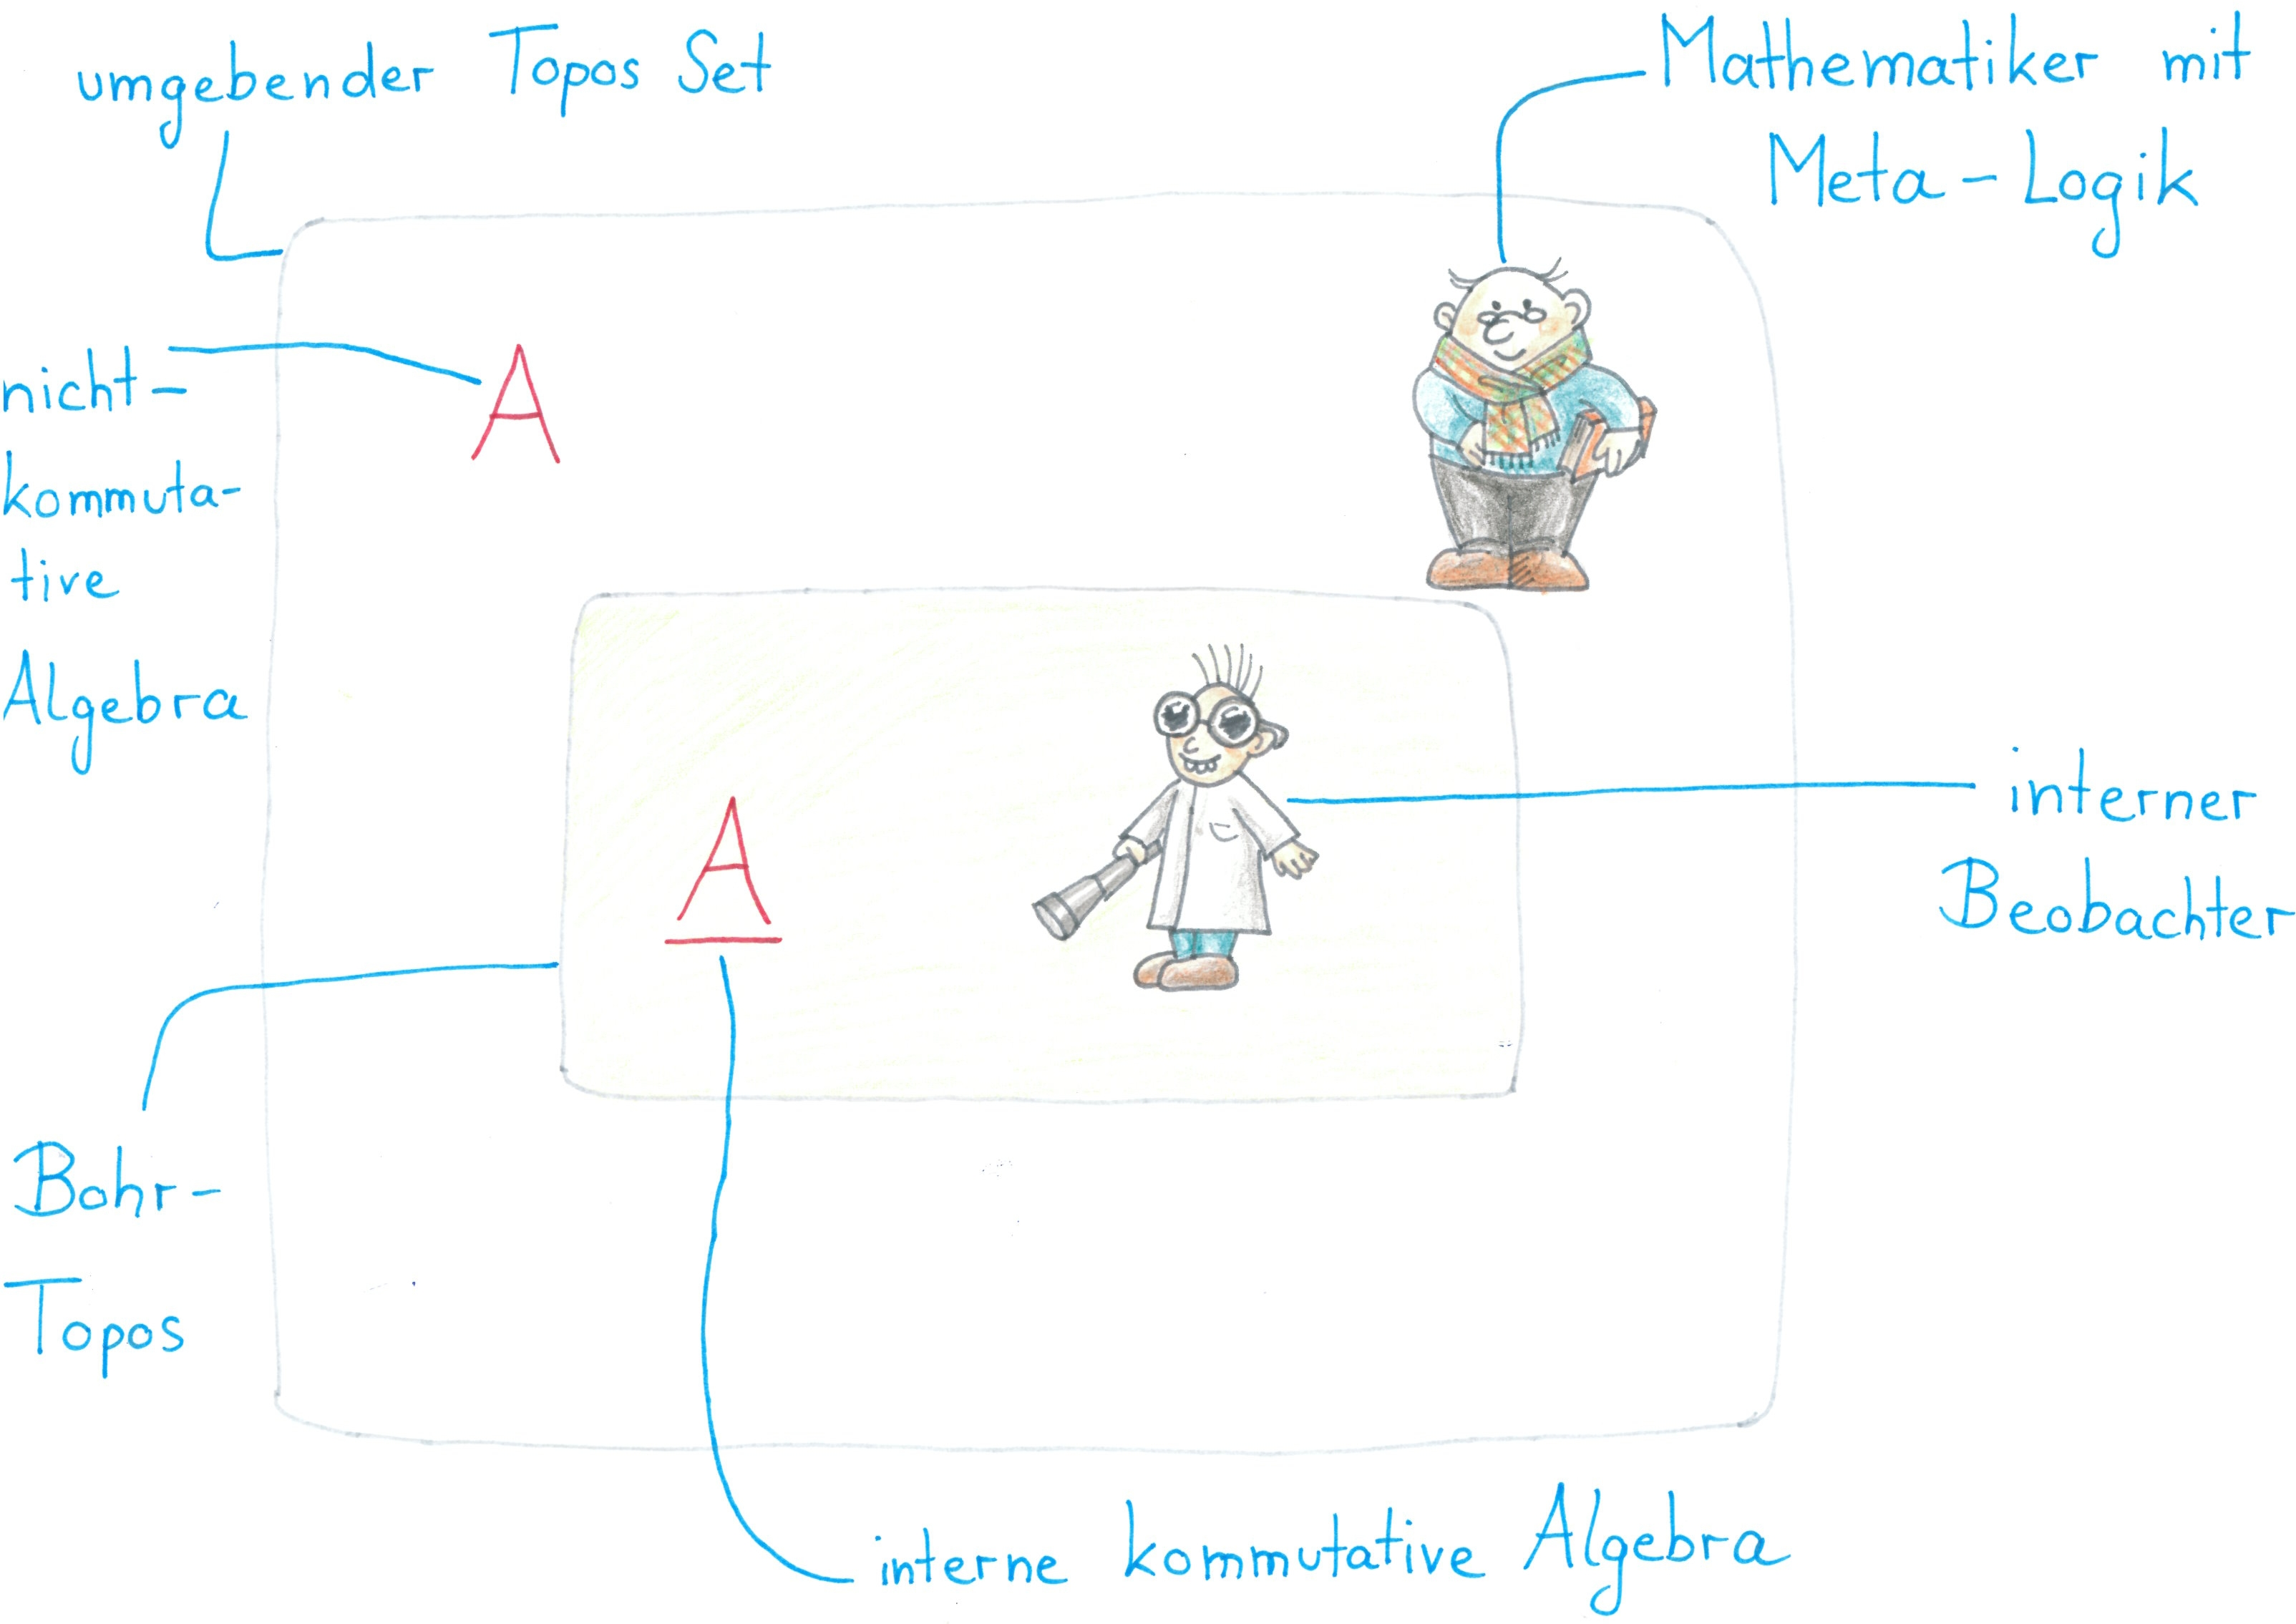
\includegraphics[width=\columnwidth]{bohr-topos}
  \end{block}
  \bigskip

  \begin{block}{Basic example}
    Let~$0 \to \F' \to \F \to \F'' \to 0$ be a short exact sequence of sheaves
    of~$\O_X$-modules. Assume that~$\F'$ and~$\F''$ are of finite type. Then it is
    well-known that~$\F$ is of finite type as well.\medskip

    A sheaf is of finite type if and only if, internally, it is a
    finitely generated module. Therefore the proposition follows \emph{at once}
    from interpreting the analogous statement of intuitionistic linear algebra
    in the little Zariski topos:
    Let~$0 \to M' \to M \to M'' \to 0$ be a short exact sequence of modules.
    Assume that~$M$ and~$M''$ are finitely generated. Then~$M$ is as well.
    \medskip

    \emph{Caveat:} Proofs by contradiction can not be interpreted with the
    internal language.
  \end{block}
\end{column}

\begin{column}{0.3\textwidth}
  \begin{block}{Locally free sheaves}
    Let~$X$ be a reduced scheme. The structure sheaf~$\O_X$ looks like a \emph{field} from the
    internal point of view. This is notable; recall that neither the rings of
    local sections nor the stalks are in general fields.\medskip

    Let~$\F$ be a finite type sheaf of~$\O_X$-modules. 
    Then it is well-known that~$\F$ is locally free on a dense open subset
    of~$X$.\medskip

    This follows \emph{at once} from the following statement of intuitionistic
    linear algebra: Let~$M$ be a finitely generated vector space. Then~$M$ is
    \emph{not not} finite free.
  \end{block}
  \bigskip

  \begin{block}{Rational functions}
    The sheaf~$\K_X$ of rational functions can internally simply be defined as
    the total quotient ring of~$\O_X$.
  \end{block}
  \bigskip

  \begin{block}{Spreading of properties}
    The following meta-theorem covers a wide range of cases:
    Let~$\varphi$ be a property which can be formulated without
    using~``$\Rightarrow$'',~``$\neg$'', and~``$\forall$''. Then~$\varphi$
    holds at a point if and only if it holds on some open neighbourhood of the
    point.\medskip

    For instance, a sheaf of modules~$\F$ is zero if and only if, from the
    internal perspective, ``$\forall x \in \F{:}\ x = 0$''. Because of
    the~``$\forall$'', a stalk may be zero without the sheaf being zero on a
    neighbourhood.\medskip

    But if~$\F$ is of finite type, the condition can be reformulated using
    generators as ``$x_1 = 0 \wedge \cdots \wedge x_n = 0$''. The meta-theorem
    is applicable to this statement, thus a stalk is zero if and only if~$\F$
    is zero on a neighbourhood.
  \end{block}

  \vspace{1cm}
  \begin{alertblock}{Dictionary external vs. internal notions}
    Detailed notes are available at \url{http://tiny.cc/topos} (work in
    progress).
  \end{alertblock}
\end{column}

\end{columns}\end{frame}

\end{document}
